\documentclass[a4paper, 12pt]{article}
\usepackage{cmap} %поиск в PDF
\usepackage[T1]{fontenc}
\usepackage[utf8]{inputenc}
\usepackage[russian]{babel}
\usepackage{multicol}
\usepackage[shortlabels]{enumitem}
\usepackage{amsmath}
\usepackage{hyperref}
\usepackage[usenames]{color}
\usepackage{colortbl}
\usepackage{amssymb}
\usepackage{tikz}
\usepackage{graphicx}
\usepackage{lipsum}
\makeatletter
\renewcommand{\@seccntformat}[1]{} %выключение нумерации секций
\makeatother
\hypersetup{
    colorlinks,
    citecolor=black,
    filecolor=blue,
    linkcolor=blue,
    urlcolor=blue
}
\usepackage[
    left=10mm,
    top=10mm,
    right=15mm,
    bottom=15mm,
]{geometry}

\def\mywidth{14}

\title{\Large{ЕЖЕНЕДЕЛЬНЫЙ НАЦИОНАЛЬНЫЙ БЮЛЛЕТЕНЬ ПО ГРИППУ И ОРВИ}}
% \date{за 7 неделю 2011 года (13.02.11 - 19.02.11)}
\author{за 1 неделю 2020 года (30.12.19 -- 05.01.20)}
\date{}

\makeatletter
\def\@maketitle{%
  \newpage
  \vspace*{-\topskip}      % remove the initial space
  \begingroup\centering    % instead of \begin{center}
  \let \footnote \thanks
  \hrule height \z@        % to avoid the insertion of lineskip glue
    {\LARGE \@title \par}%
    \vskip 0.1em 
    {\large
      \lineskip .3em 
      \begin{tabular}[t]{c}%
        \@author
      \end{tabular}\par}%
    \vskip 0.5em 
    {\large \@date}%
  \par\endgroup            % instead of \end{center}
  \vskip 1em             % <--- modify this to adjust the separation
}
\makeatother

\begin{document}
\maketitle
% \section*{Эпидемиологические данные}
% \subsection*{Прогноз}

На момент 1 недели 2020 года количество зарегистрированных случаев заболеваний составляет 3683 человек среди населения младше 15 лет, и 4109 человек с возрастом 15
лет и старше. На прошлой неделе аналогичные показатели составляли 13688 и 15589 человек соответственно. Таким образом, среди возрастной 
группы 0-14 лет количество зарегистрированных случаев заболеваний уменьшилось на 10005 чел. (73.1 \%), а среди возрастной группы 15 лет и старше -- уменьшилось на 11480 чел. (73.6 \%) 
по сравнению аналогичными показателями на прошлой неделе. 
\maketitle
\begin{figure}[!ht]
    \centering
    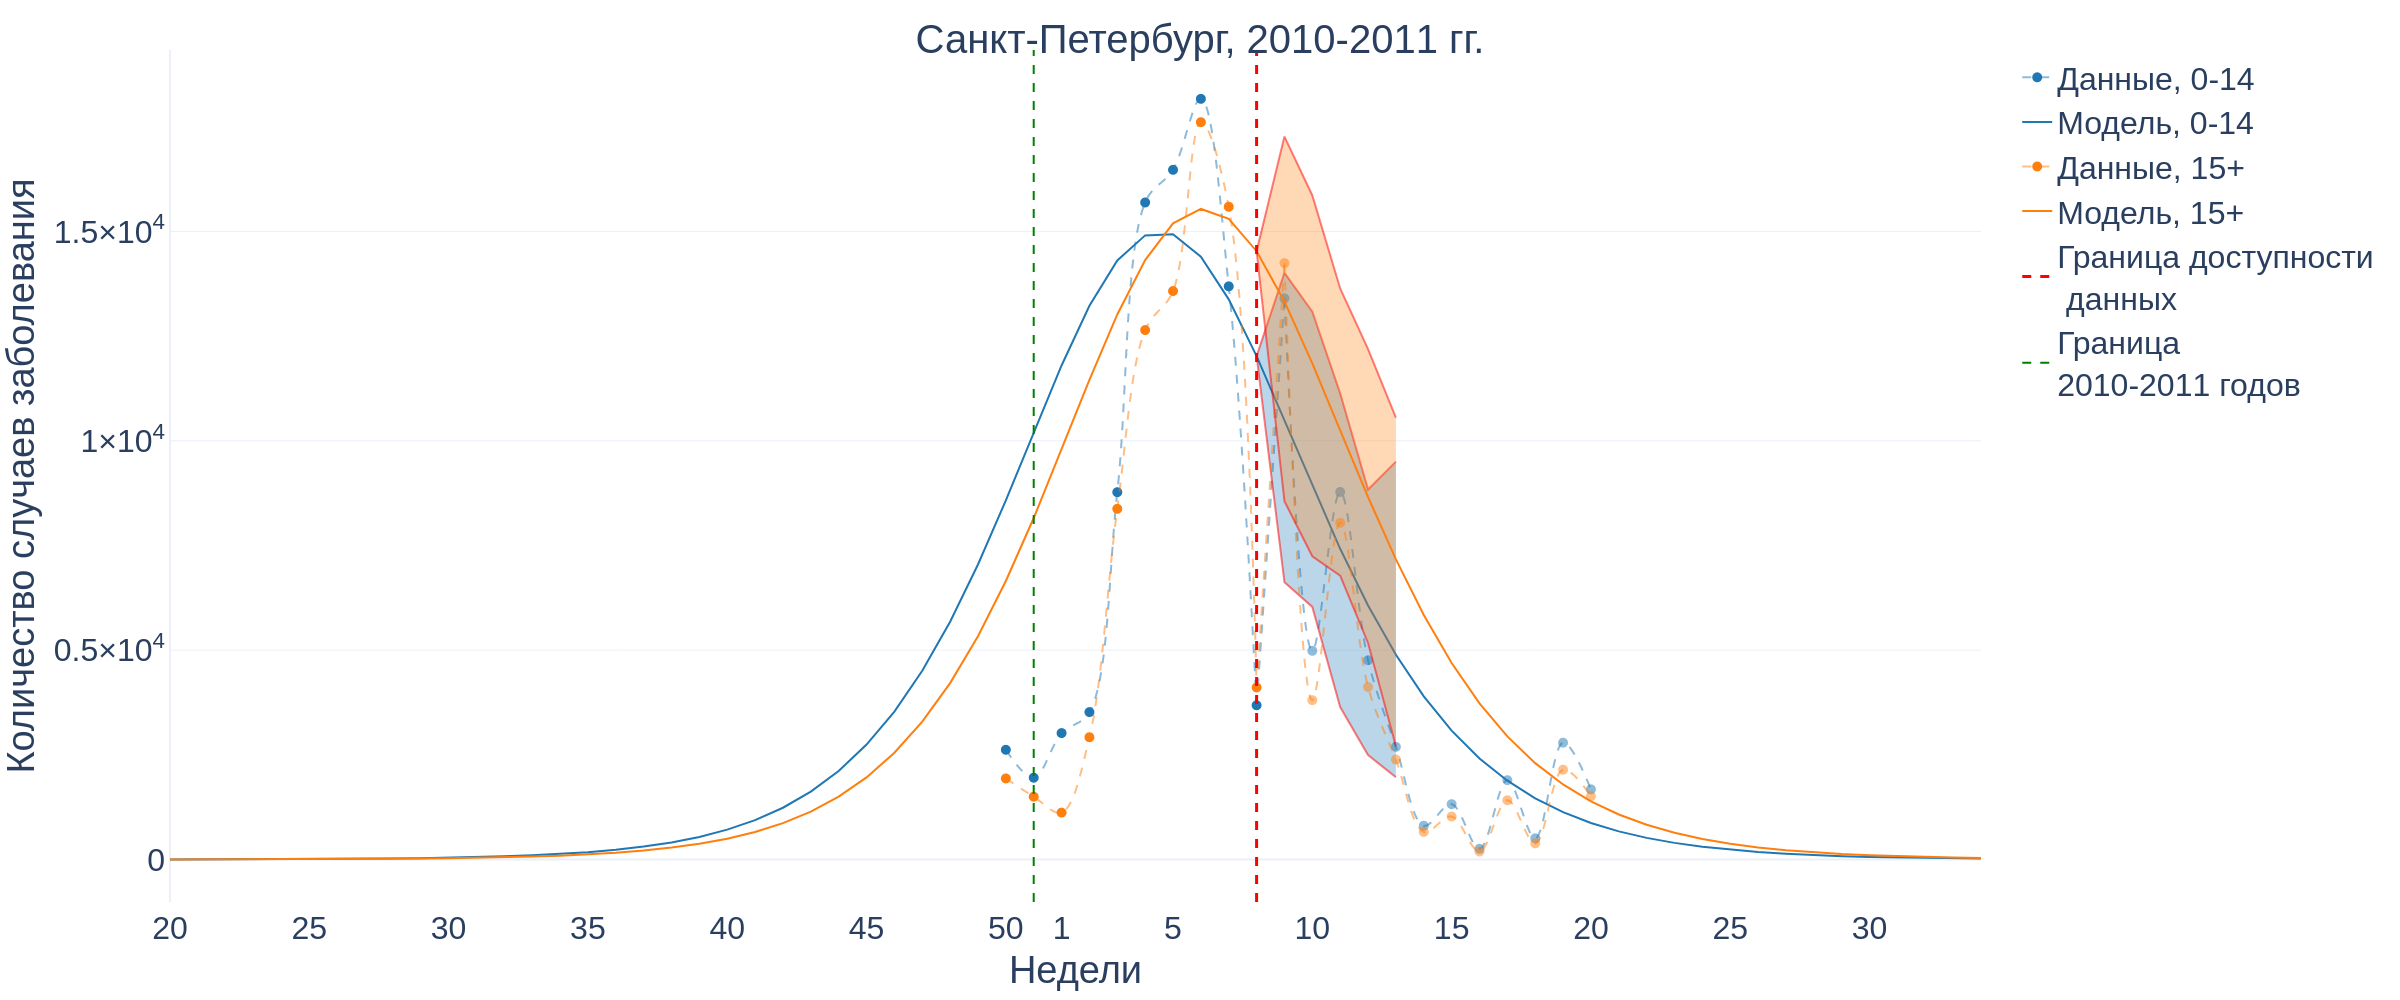
\includegraphics[width=\mywidth cm]{age-group_forecast.png}
    \caption{Прогноз заболеваемости по возрастным группам, границы доверительного интервала для $p = 0.95$}
    \label{fig:enter-label}
\end{figure}

% \begin{figure}[!ht]
%     \centering
%     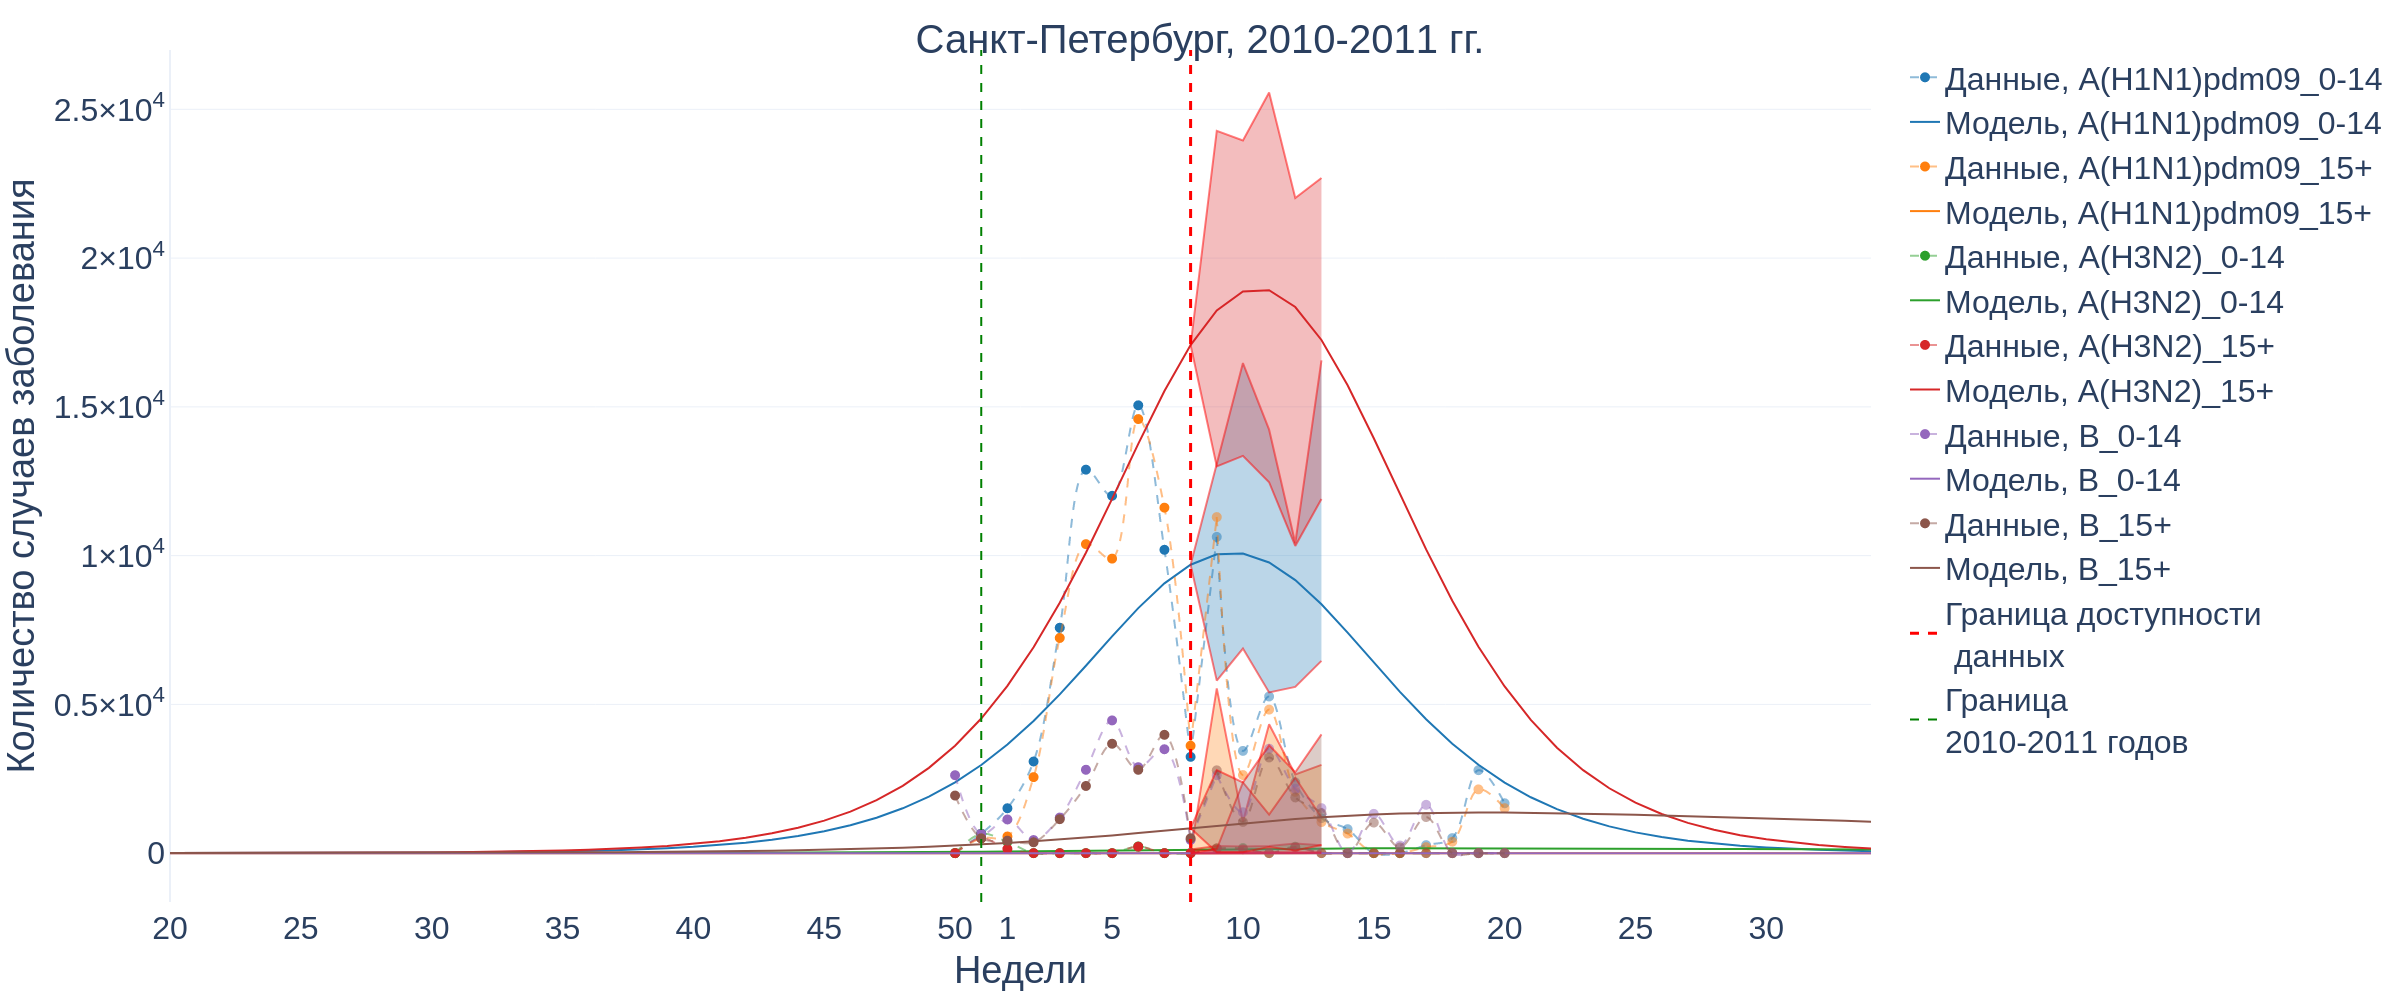
\includegraphics[width=\mywidth cm]{strain_age-group_forecast.png}
%     \caption{Прогноз заболеваемости по возрастным группам и штаммам, границы доверительного интервала для $p = 0.95$}
%     \label{fig:enter-label}
% \end{figure}


% \begin{figure}[!ht]
%     \centering
%     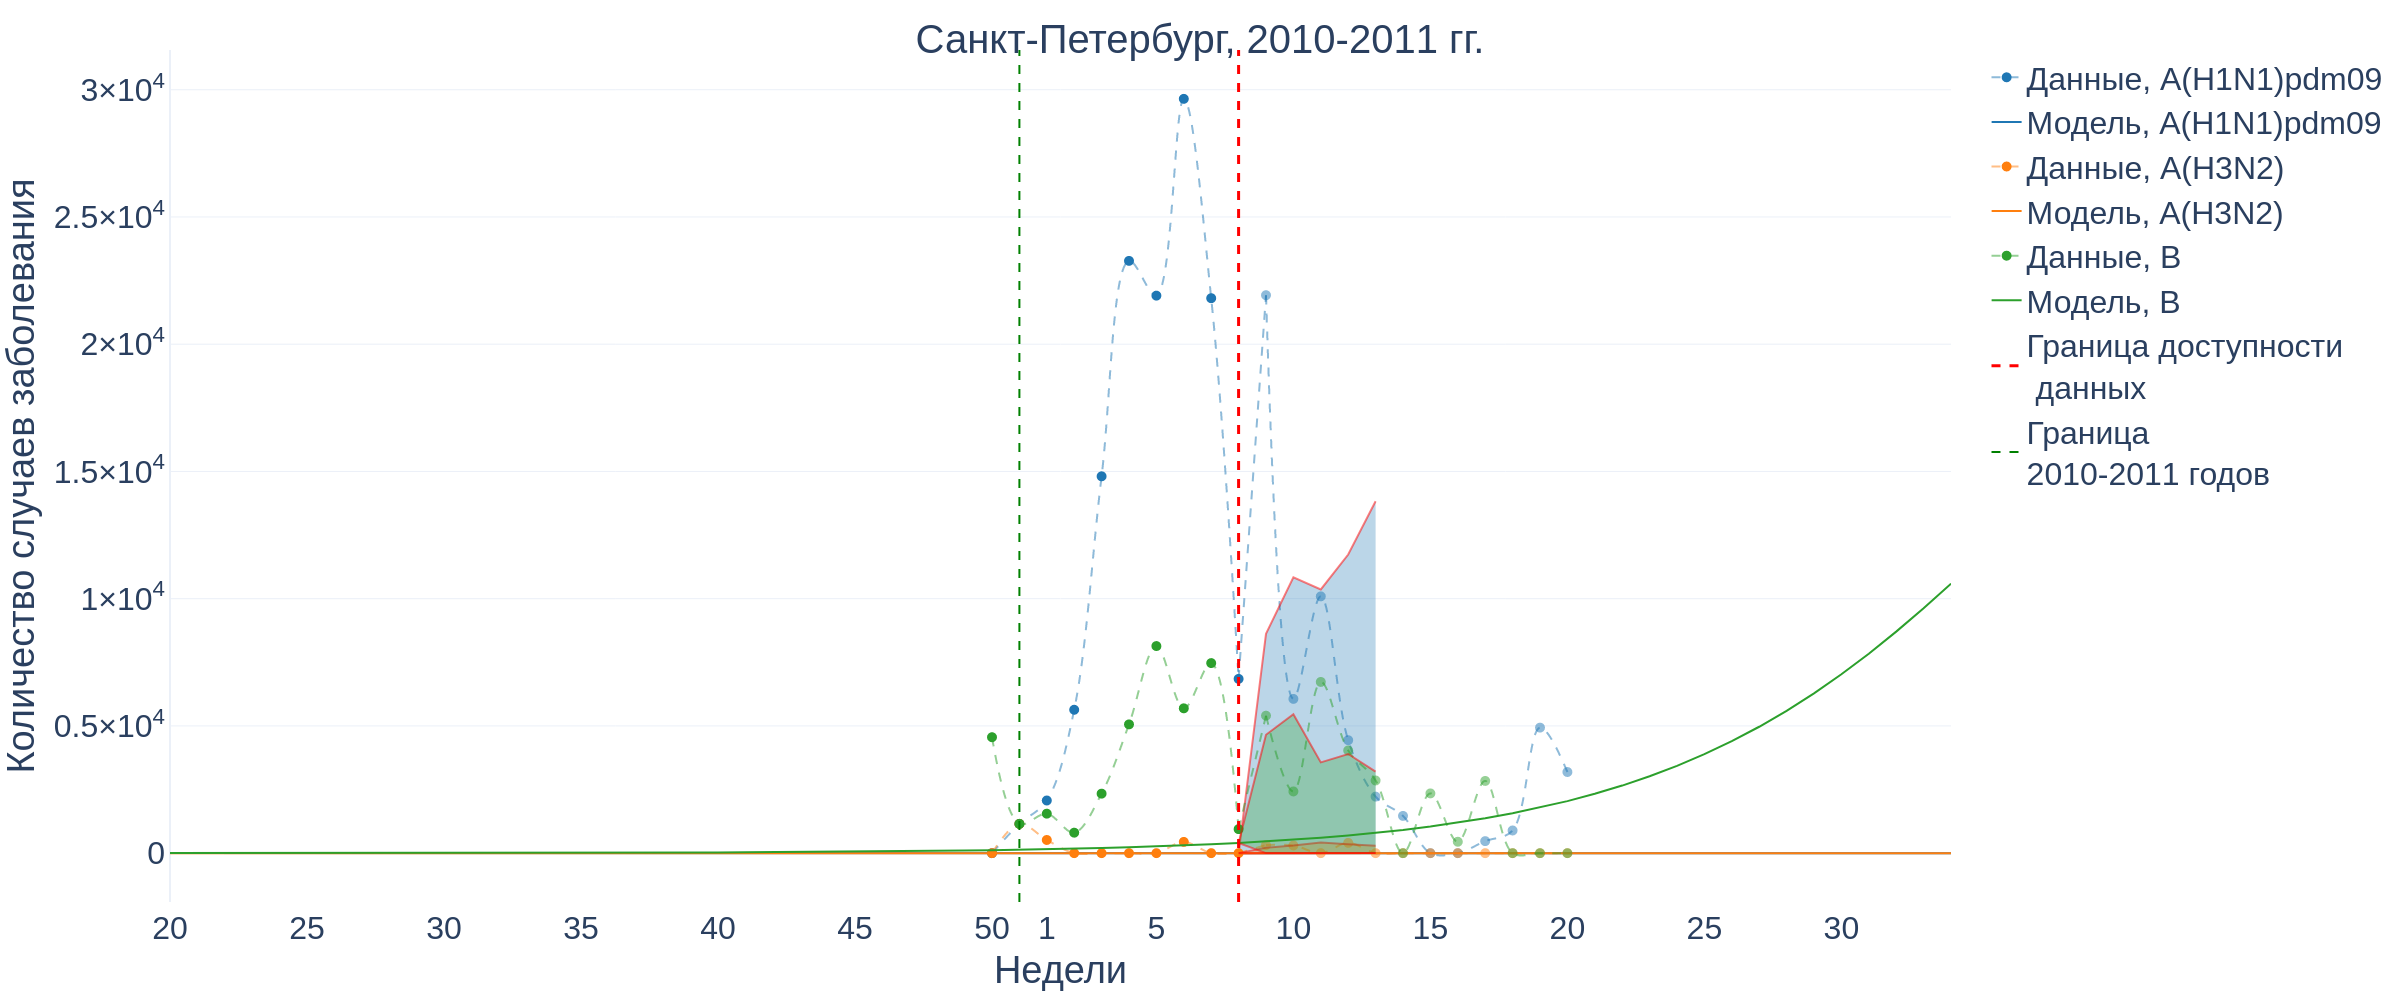
\includegraphics[width=\mywidth cm]{strain_forecast.png}
%     \caption{Прогноз заболеваемости по различным штаммам, границы доверительного интервала для $p = 0.95$}
%     \label{fig:enter-label}
% \end{figure}


% \begin{figure}[!ht]
%     \centering
%     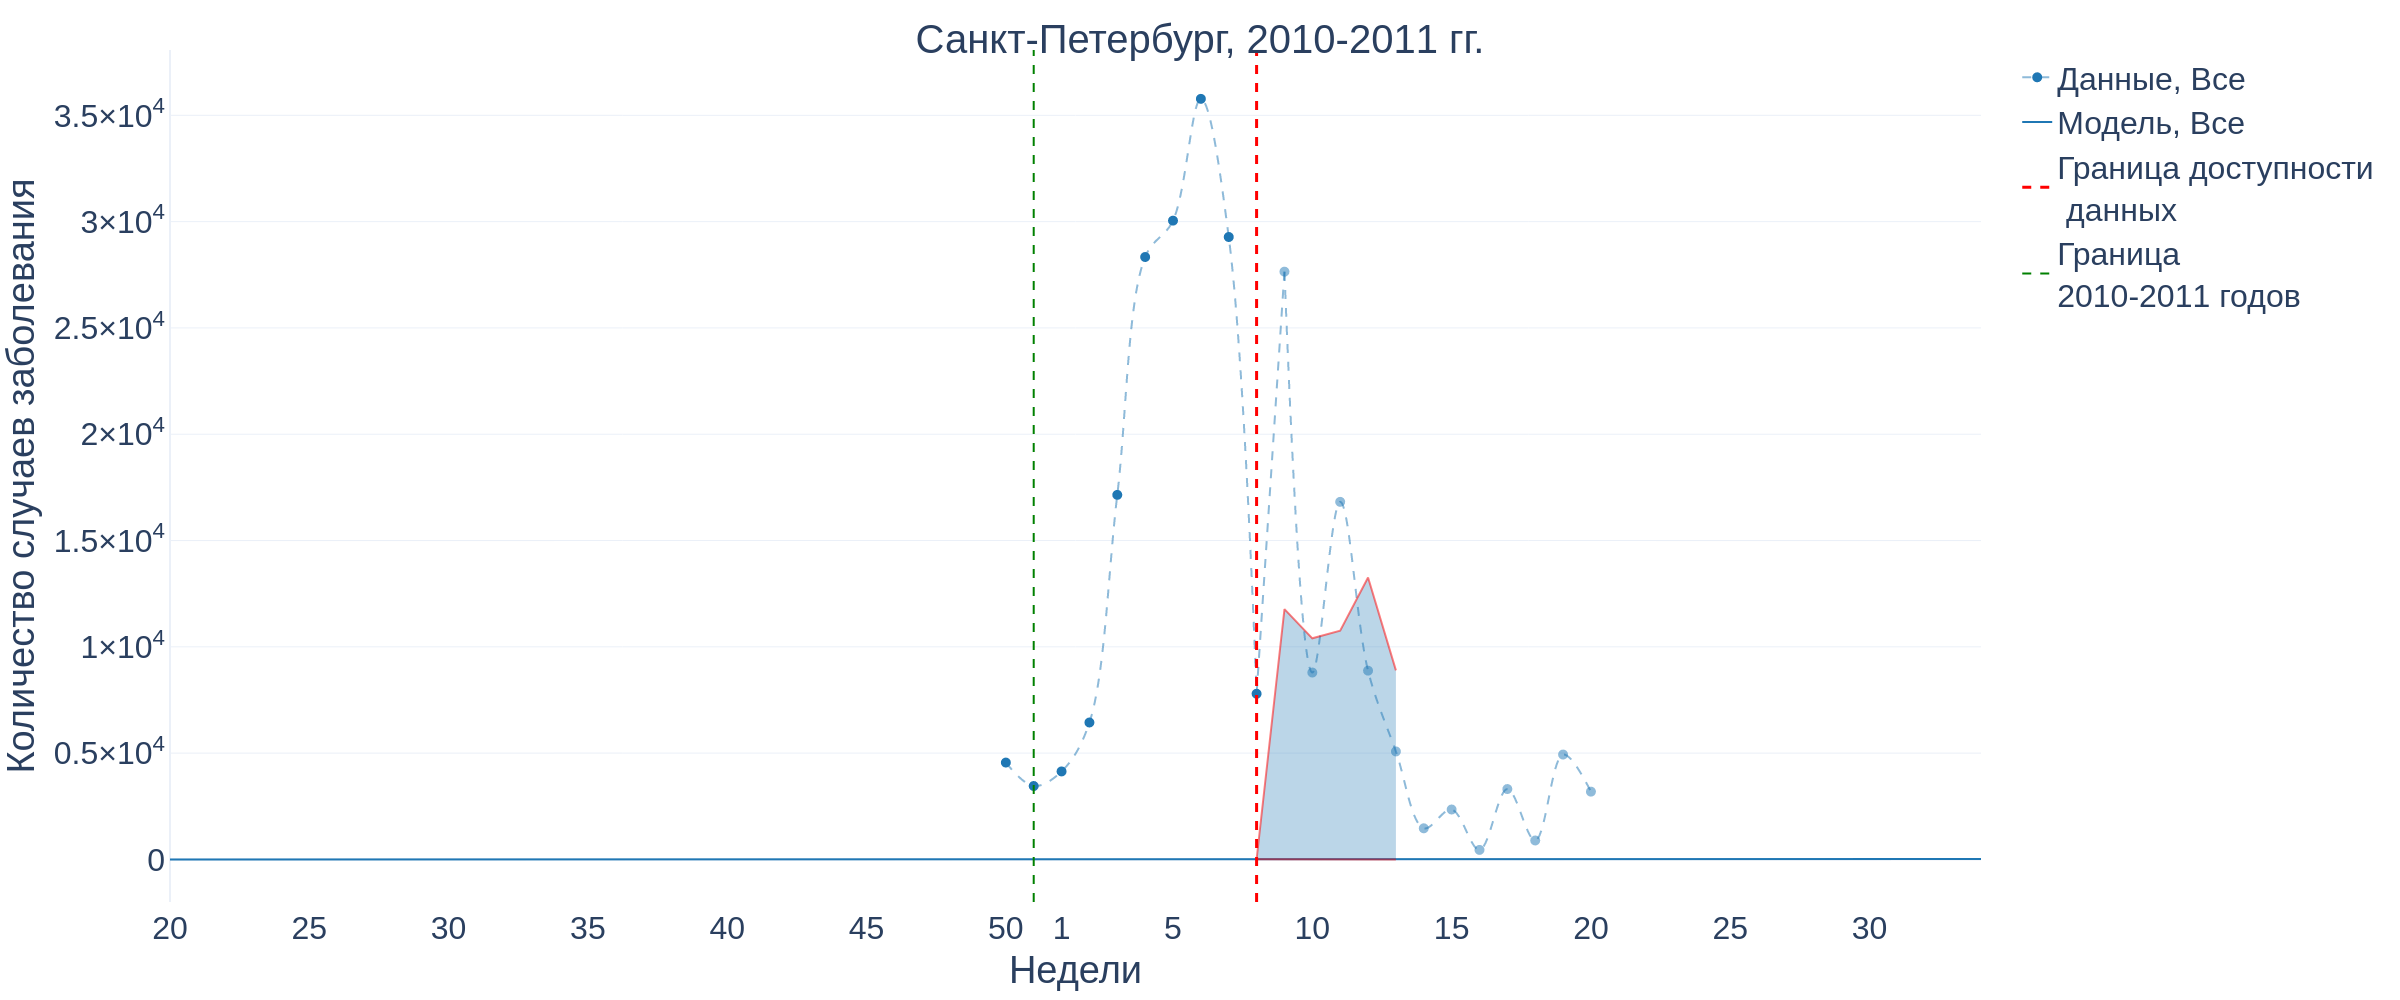
\includegraphics[width=\mywidth cm]{total_forecast.png}
%     \caption{Прогноз заболеваемости для всего населения}
%     \label{fig:enter-label}
% \end{figure}

% \clearpage
% \section*{Резюме}
% \lipsum[1]

% \clearpage
% \subsection*{Модель}
% \begin{figure}[!ht]
%     \centering
%     \includegraphics[width=\mywidth cm]{age-group.png}
%     \caption{Данные по заболеваемости по возрастным группам}
%     \label{fig:enter-label}
% \end{figure}

% \begin{figure}[!ht]
%     \centering
%     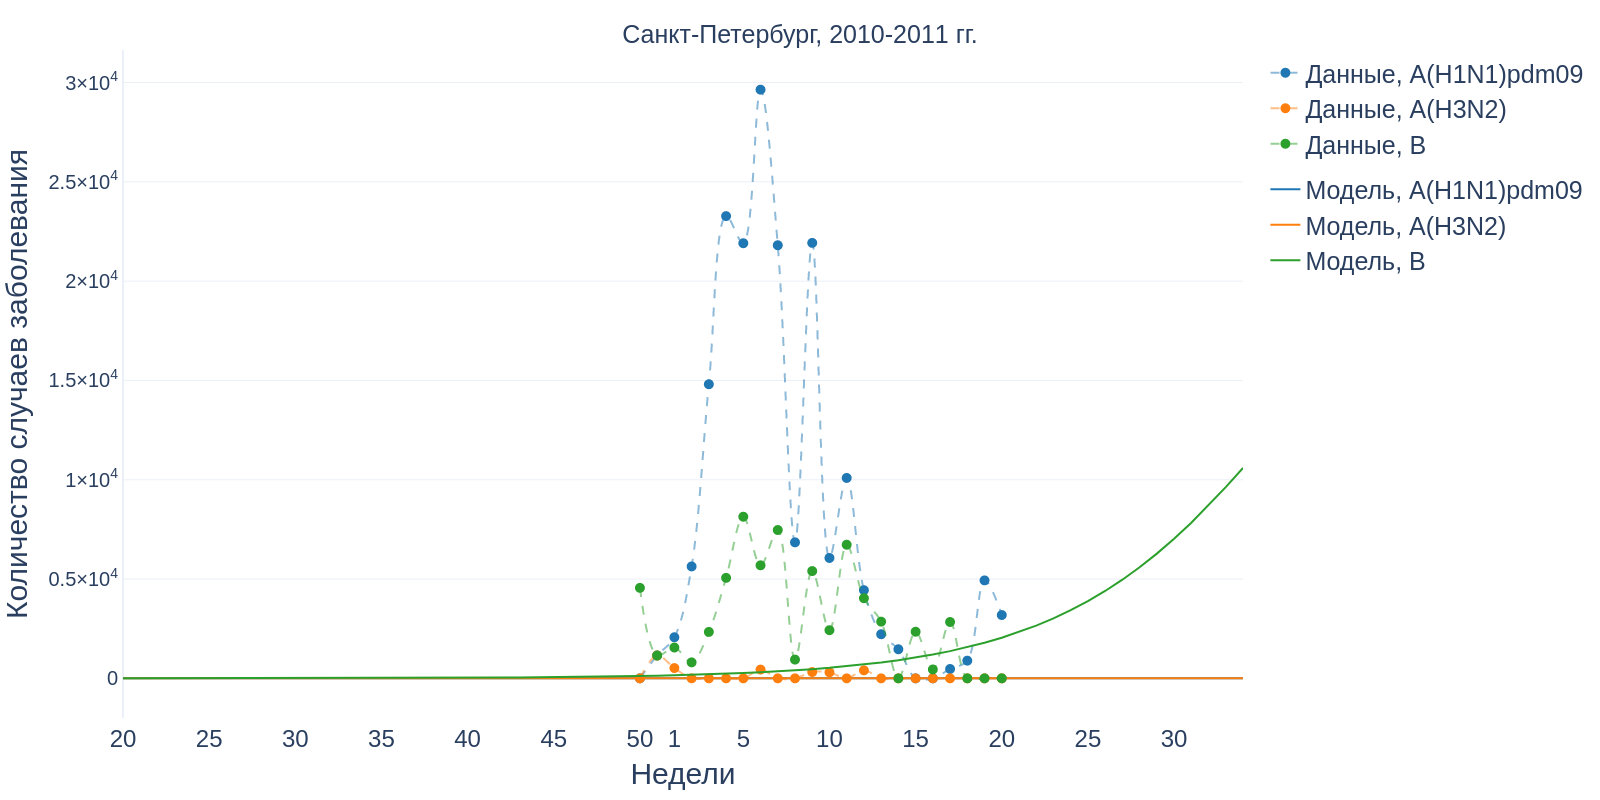
\includegraphics[width=\mywidth cm]{strain.png}
%     \caption{Данные по заболеваемости по различным штаммам}
%     \label{fig:enter-label}
% \end{figure}

% \begin{figure}[!ht]
%     \centering
%     \includegraphics[width=\mywidth cm]{strain_age-group.png}
%     \caption{Данные по заболеваемости по возрастным группам и штаммам}
%     \label{fig:enter-label}
% \end{figure}

% \begin{figure}[!ht]
%     \centering
%     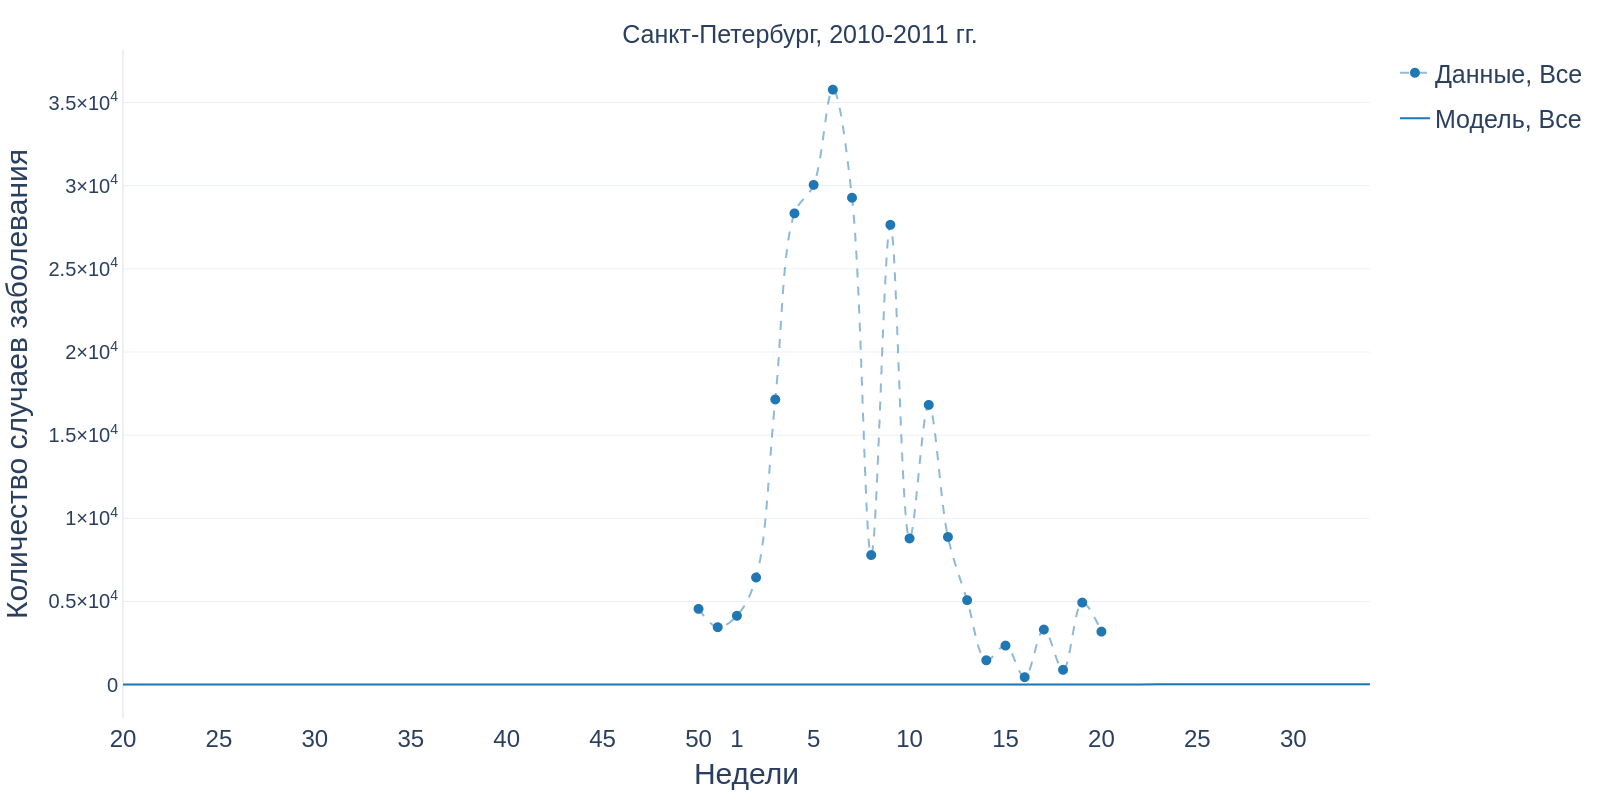
\includegraphics[width=\mywidth cm]{total.png}
%     \caption{Данные по заболеваемости для всего населения}
%     \label{fig:enter-label}
% \end{figure}

\end{document}
    

